\section{מבוא}

\subsection{רקע כללי: האתגר בבקרת אקלים ובית שורשים}
החקלאות המודרנית ניצבת בפני אתגר כפול: הצורך למקסם את היבול ליחידת שטח, תוך צמצום השימוש במשאבים (מים ודשן) ומזעור ההשפעה הסביבתית. בחממות טכנולוגיות, המבוססות לרוב על מצעים מנותקים, השליטה על תנאי בית השורשים \LR{(Rootzone)} היא המפתח להשגת מטרות אלו. בניגוד לגידולי שדה בקרקע טבעית, למצע המנותק יש באפר קיבול \LR{(Buffering Capacity)} נמוך, ומשמעות הדבר היא שכל טעות בדישון או בהשקיה משפיעה באופן מידי וחריף על הצמח.

בסביבה דינמית זו, שני המדדים הקריטיים ביותר לניטור הם:

\begin{itemize}
    \item \textbf{מוליכות חשמלית \LR{(EC)}:} מדד המייצג את סך המלחים המומסים בתמיסה. שמירה על רמת EC אופטימלית היא איזון עדין -- ערך נמוך מדי יגרום לחוסר הזנה ופגיעה בקצב הצימוח, בעוד שערך גבוה מדי ייצור לחץ אוסמוטי שיקשה על הצמח לקלוט מים, ואף עלול לגרום לצריבות והמתקת יבול מוקדמת.
    \item \textbf{חומציות \LR{(pH)}:} מדד הקובע את המסיסות והזמינות של יסודות ההזנה (בעיקר מיקרו-אלמנטים כמו ברזל ומנגן). סטייה ב-pH עלולה להוביל למצבי חוסר (Deficiency) או רעילות (Toxicity) גם אם הדשן סופק בכמות הנכונה.
\end{itemize}

\subsection{הפער בין הרצוי למצוי בניטור}
על אף החשיבות הקריטית של מדדים אלו, קבלת תמונת מצב אמינה ורציפה של בית השורשים מהווה כיום "צוואר בקבוק" טכנולוגי. המגדל נדרש לבחור בין שתי חלופות שאינן מושלמות:

\textbf{דגימות מעבדה ידניות \LR{(Manual Sampling)}:} זוהי שיטת ה־\LR{Gold Standard} מבחינת דיוק. דגימת נקז או מיצוי מצע נבדקת במכשיר מעבדה מכויל. עם זאת, שיטה זו דורשת כוח אדם וזמן, ולכן מתבצעת לרוב בתדירות נמוכה (אחת ליום או למספר ימים). התוצאה היא "נקודות עיוורות" בזמן; ייתכן שבין שתי דגימות תקינות התרחש אירוע קיצון של המלחה \LR{(Spike)} שגרם לנזק בלתי הפיך, אך לא תועד. כמו כן, שיטה זו היא ריאקטיבית (תגובתית) -- המידע מתקבל לאחר מעשה.

\begin{figure}[H]
    \centering
    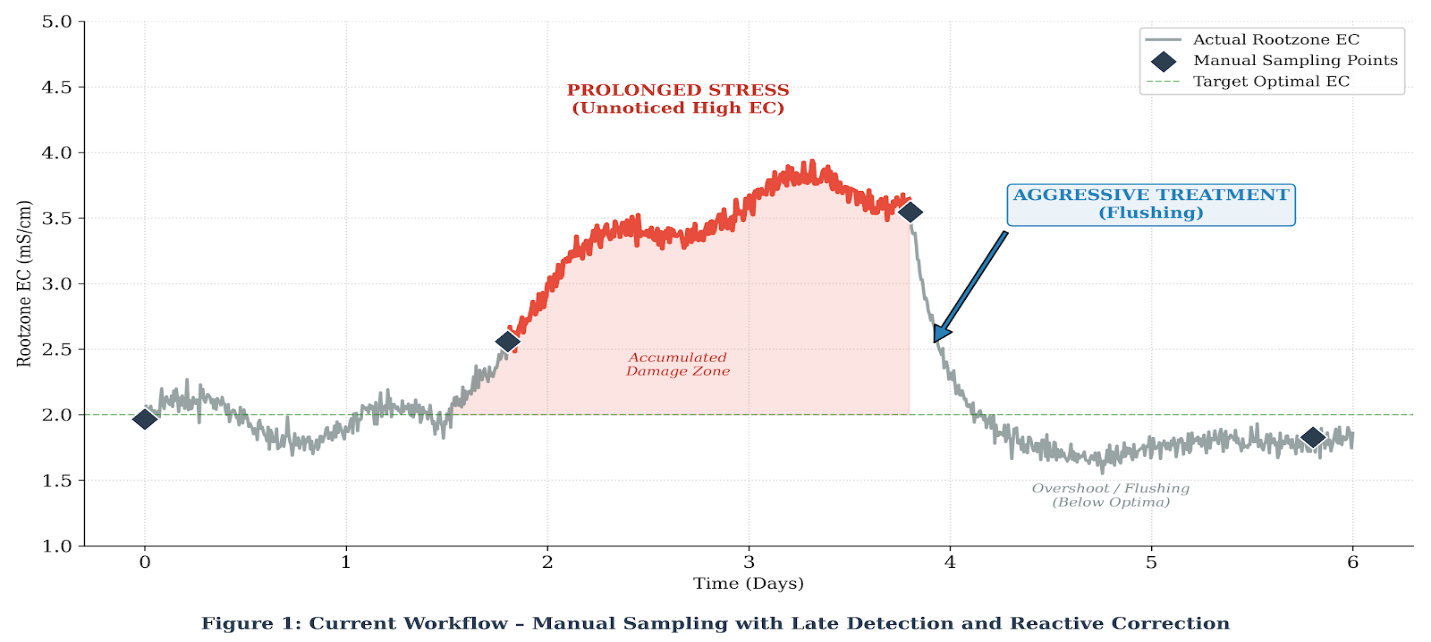
\includegraphics[width=0.92\textwidth]{figures/fig01.png}
    \caption{\LR{Current Workflow -- Manual Sampling with Late Detection and Reactive Correction}}
    \label{fig:workflow}
\end{figure}

איור \ref{fig:workflow} ממחיש תרחיש טיפוסי: מליחות בית השורשים חורגת מהטווח האופטימלי בין שתי דגימות ידניות, נשארת גבוהה לאורך פרק זמן ממושך ("אזור נזק מצטבר"), ומזוהה רק בדגימה המאוחרת -- מה שמחייב טיפול אגרסיבי (שטיפה) לתיקון המצב.

\textbf{חיישני קרקע רציפים \LR{(In-situ Sensors)}:} חיישנים אלו מספקים רצף נתונים \LR{(Time-Series)} ומאפשרים זיהוי מגמות בזמן אמת. אולם, השימוש בהם טומן בחובו אתגרים טכניים משמעותיים:

\begin{itemize}
    \item \textbf{סחיפה וכיול \LR{(Drift \& Calibration)}:} האלקטרודות נוטות לצבור משקעים וביופילם, הגורמים לקריאה "לנדוד" עם הזמן ולספק נתונים שגויים.
    \item \textbf{ייצוגיות מרחבית:} חיישן מודד נקודה בודדת במרחב. בחממה גדולה, או אפילו בתוך עציץ בודד, קיימת שונות מרחבית גבוהה ברטיבות ובמליחות. חיישן הממוקם ליד הטפטפת יראה ערך שונה לחלוטין מחיישן הממוקם בתחתית המצע.
    \item \textbf{עלות:} פריסה רחבה של חיישנים איכותיים דורשת השקעה כספית גבוהה ותחזוקה שוטפת.
\end{itemize}

\subsection{הבסיס הפיזיקלי-ביולוגי}
הקושי בחיזוי משתני השורשים נובע מכך שבית השורשים הוא מערכת דינמית המושפעת ממאזן מסה \LR{(Mass Balance)} משתנה. הצמח קולט מים ודשן בקצבים שונים:

\begin{itemize}
    \item \textbf{בימים של קרינה גבוהה:} הצמח מבצע דיות (Transpiration) מוגברת ו"שותה" בעיקר מים נקיים, מה שמותיר את המלחים במצע ועשוי לגרום לעליית EC מהירה.
    \item \textbf{בימים מעוננים:} קצב הדיות יורד, וצריכת המים והדשן מתאזנת.
\end{itemize}

המודל שלנו נועד ללמוד את הדפוסים הללו (הקשר הלא-ליניארי בין קרינה לצריכת מים) ולחזות את הצטברות המלחים שנובעת מהם.

\begin{figure}[H]
    \centering
    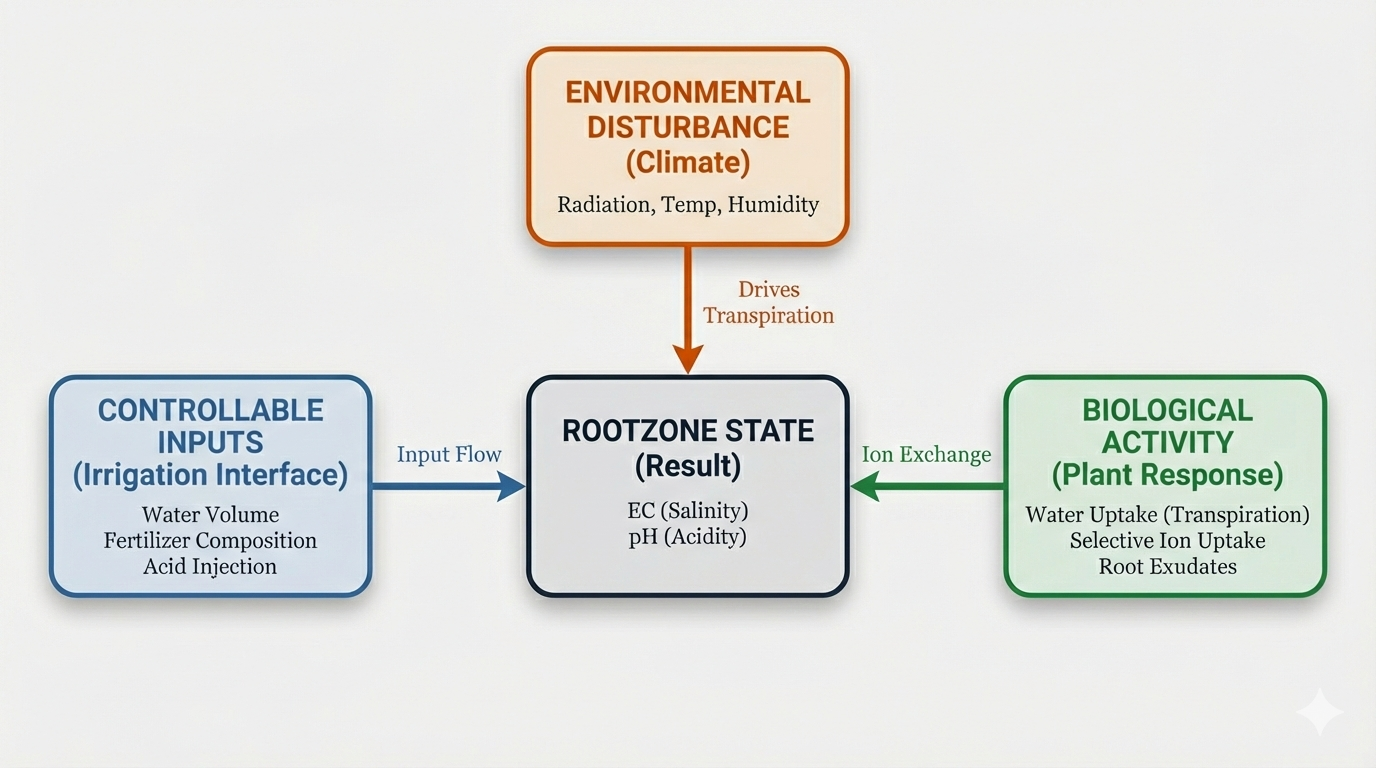
\includegraphics[width=0.85\textwidth]{figures/fig02.png}
    \caption{\LR{Physical-Biological Basis of Rootzone Dynamics}}
    \label{fig:physbio}
\end{figure}

כפי שמתואר באיור \ref{fig:physbio}, מצב בית השורשים הוא תוצאה של שילוב בין הפרעה סביבתית (אקלים, המניעה דיות), קלטים בני-שליטה (השקיה, דישון, חומצה) ופעילות ביולוגית של הצמח (קליטת מים וחילופי יונים).

\subsection{למה למידת מכונה?}
באופן מסורתי, ניתן לחזות תהליכים אלו באמצעות משוואות פיזיקליות מורכבות. אולם, מודלים אלו דורשים פרמטרים רבים שקשה מאוד למדוד בשטח (כגון מוליכות הידראולית של המצע, נקבוביות משתנה ושטח פנים של השורשים). גישת למידת המכונה \LR{(Data-Driven Approach)} עוקפת את הצורך במדידת הפרמטרים הללו. המודל אינו מחליף את ההבנה הפיזיקלית, אלא לומד קשרים אמפיריים מתוך הנתונים -- המודל לומד את ההתנהגות האפקטיבית של המערכת ישירות מתוך הנתונים ההיסטוריים, ובכך מאפשר דיוק גבוה בעלות חישובית נמוכה.

\subsection{הפתרון המוצע: "חיישן תוכנה" מבוסס נתונים}
פרויקט זה מציע גישה המבוססת על תפיסת ה־\LR{Soft Sensing} ("חיישן תוכנה"), שמטרתה להעריך את מצב בית השורשים גם בפרקי הזמן שבהם לא קיימת מדידה ישירה. ההנחה המרכזית היא שקיים קשר פיזיקלי-כימי בין תנאי הסביבה החיצוניים, המיקרו-אקלים בתוך החממה, פעולות המגדל כגון השקיה ודישון, ומדדי התגובה בבית השורשים.

באמצעות אלגוריתמים של למידת מכונה ניתן ללמוד קשרים מורכבים ובלתי ליניאריים אלו מתוך הנתונים ההיסטוריים, ולייצר תחזית של ערכי pH ו-EC על בסיס מידע זמין כגון נתוני אקלים, השקיה, דישון ומדידות עבר. גישה זו אינה מחליפה את המדידות הידניות המדויקות, אלא משלימה אותן ומסייעת לצמצם את פערי המידע בין מועדי הדגימה.

\subsection{מטרות הפרויקט}

\begin{itemize}
    \item \textbf{אינטגרציית נתונים:} יצירת מסד נתונים מאוחד \LR{(Master Dataset)} המשלב ומנרמל מקורות מידע הטרוגניים, ובהם נתוני אקלים חיצוני, נתוני מיקרו-אקלים בחממה, נתוני השקיה ודישון, משתני מצב הצמח ומדידות ידניות של pH ו-EC.
    \item \textbf{פיתוח מודל חיזוי לבית השורשים:} בניית מודל למידת מכונה המסוגל לחזות את ערכי ה-pH וה-EC בנקודת זמן עתידית, על בסיס מדידה נוכחית ידועה, תנאי הסביבה, פעולות ההשקיה והדישון, ומצב הצמח בפרק הזמן הרלוונטי. מטרת המודל היא לשמש כ־\SoftSensor{} המאפשר הערכת מצב רציפה יותר של בית השורשים בין מדידות ידניות דלילות.
    \item \textbf{שילוב בין למידה מדפוסים לבין חיזוי מגמות:} פיתוח גישה היברידית המשלבת מודל \GB{}, הלומד דפוסים מורכבים מתוך נתוני העבר, עם רכיב ליניארי חסין המסייע בהתמודדות עם אירועים תפעוליים חריגים או בעלי השפעה גבוהה. שילוב זה נועד לאפשר גם אינטרפולציה בתוך תחומי התנהגות מוכרים וגם אקסטרפולציה זהירה במצבים שבהם נדרשת תגובה לשינוי חד.
    \item \textbf{ולידציה בתנאי אמת:} בחינת ביצועי המודל באמצעות \WFV{} ובדיקות Holdout על מרווחים מדולגים, באופן המדמה תרחיש תפעולי שבו המודל מאומן על נתוני עבר ונדרש לחזות נקודות עתידיות. מטרת הוולידציה היא להעריך את יציבות המודל ואת התאמתו לשימוש ככלי תומך החלטה לניהול השקיה ודישון.
\end{itemize}
